\documentclass[14pt, a4paper]{report}
\usepackage{mathtext}
\usepackage[T2A]{fontenc}
\usepackage[utf8]{inputenc}
\usepackage[russian]{babel}
\usepackage{multirow}
\usepackage{slashbox}
\usepackage{makecell}
\usepackage{graphicx}
\usepackage{physics}
\usepackage{amstext}
\usepackage{caption}
\usepackage{subcaption}
\usepackage{cmap}
\usepackage{float}
\usepackage{siunitx}
\usepackage{wrapfig}

\renewcommand{\thesection}{\arabic{section}.}
\renewcommand{\thesubsection}{\arabic{section}.\arabic{subsection}.}

\title{\textbf{Отчет о выполнении лабораторной работы 4.3.1 "Дифракция света"}}
\author{Калашников Михаил, Б03-205}
\date{}

\begin{document}
\maketitle

\textbf{Цель работы:}
исследовать явления дифракции Френеля и Фраунгофера на одной и двух щелях, изучить влияние дифракции на разрешающую способность оптических инструментов; проверить теоретические соотношения для положения максимумов при дифракции Френеля и Фраунгофера.
\newline

\textbf{В работе используются:}
\begin{itemize}
\item оптическая скамья;
\item ртутная лампа;
\item светофильтр;
\item щели с регулируемой шириной;
\item рамка с вертикальной нитью;
\item экран с двойной щелью;
\item микроскоп на поперечных салазках с микрометрическим винтом;
\item зрительная труба.
\end{itemize}

\section{Теоретические сведения}

\paragraph{Дифракция Френеля}
Суммарное ширина $n$ зон Френеля $z_n$ определяется соотношением 
\begin{equation}
    z_n = \sqrt{an\lambda}
\end{equation}
где $n$ -- номер зоны, $a$ -- расстояние от щели до плоскости наьлюдений, $\lambda$ -- длина волны. В работе используется ртутная лампа с длиной волны $\lambda = 5461 \cdot 10^{-10}$ м.

\paragraph{Дифракция Фраунгофера}
При дифракции Фраунгофера на одной щели имеет место соотношение
\begin{equation}
    X_m = m f_2 \frac{\lambda}{D}
\end{equation}
где $X_m$ -- расстояние темной полосы от оптическое оси объектива, $f_2$ -- фокусное расстояние линзы, $m$ -- номер темной полосы, $D$ -- ширина щели. \\
При дифракции Фраунгофера на двух щелях будем пользоваться соотношением 
\begin{equation}
    \delta x = f_2 \frac{\lambda}{d} = \frac{2d}{Dn}
\end{equation}
где $\delta x$ -- линейное расстояние между соседними интерференционными полосами в плоскости наблюдения, $n$ -- число темных полос в центральном максимуме.

\paragraph*{А. Дифракция Френеля}

\section{Настройка установки}

\begin{enumerate}

\item Настроим зрительную трубу на бесконечность.

\item Определим нуль микрометрического винта щели $S_2$.

\item Соберем схему установки для наблюдения дифракции Френеля.

\item Проверим, что при небольшом удалении микроскопа от щели на ярком фоне геометрического изображения щели появляются узкие темные дифракционные полосы, количество которых уменьшается по мере удаления микроскопа.

\item Попытаемся улучшить контрастность картины с помощью регулирования ширины щели $S_1$.

\end{enumerate}

\begin{figure}[H]
\centering
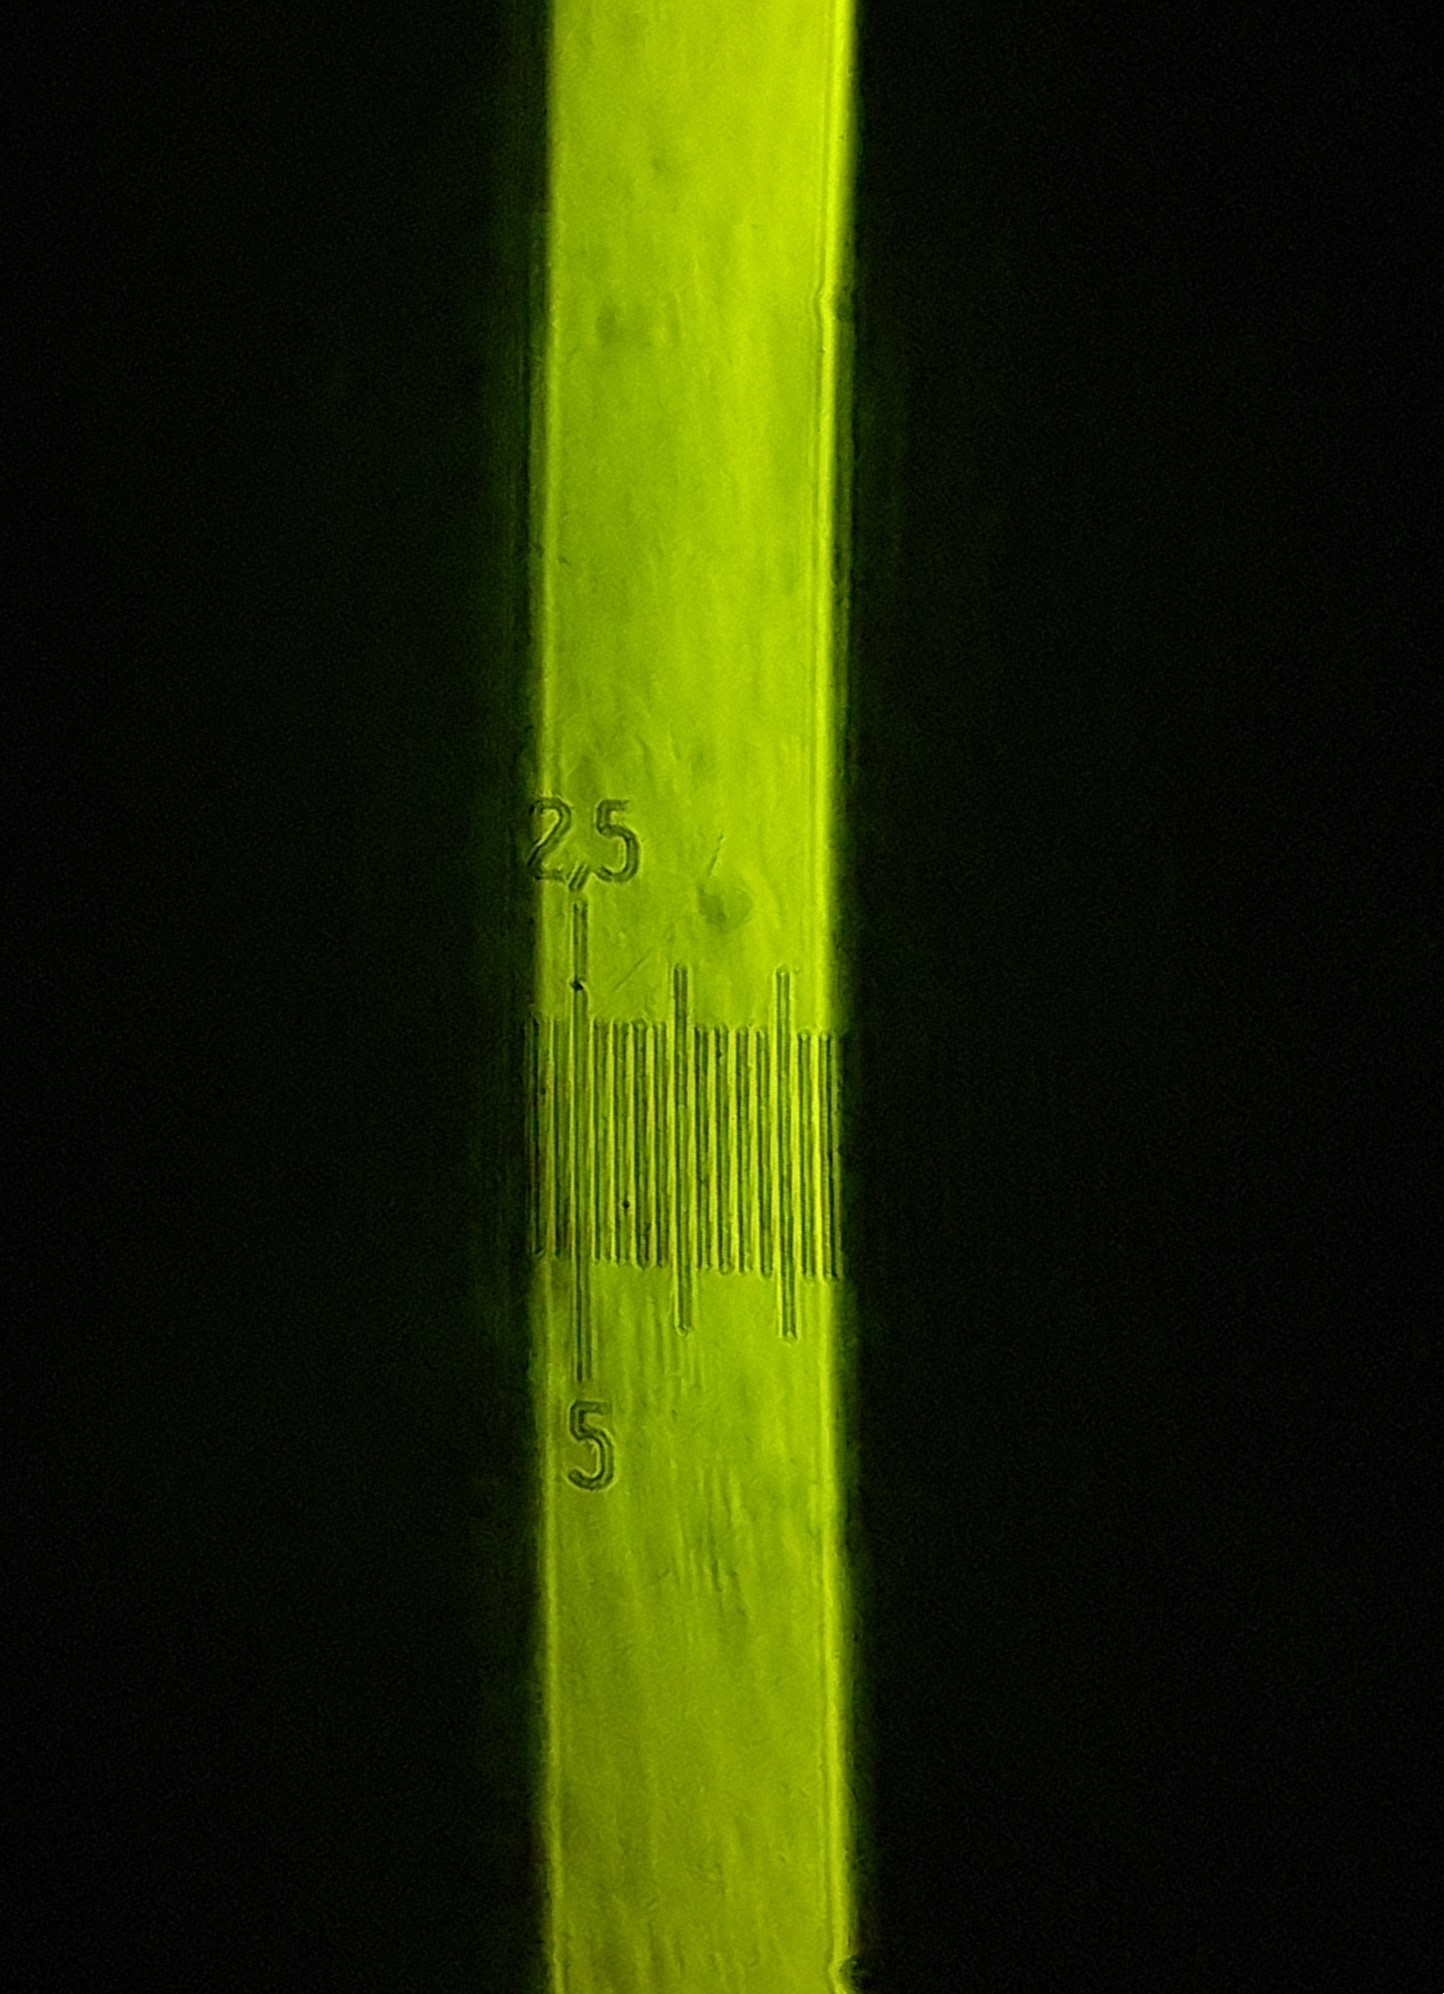
\includegraphics[scale=0.2]{../images/431m_1}
\end{figure}

\section{Проведение измерений}

\begin{enumerate}

\item Вновь найдем резкое изображение щели. Запишем начальное положение микроскопа.

\item Постепенно отодвигая микроскоп от щели $S_2$, заметим по шкале положение, при котором на фоне видна одно темная полоса.

\begin{figure}[H]
\centering
\begin{minipage}{.33\textwidth}
  \centering
  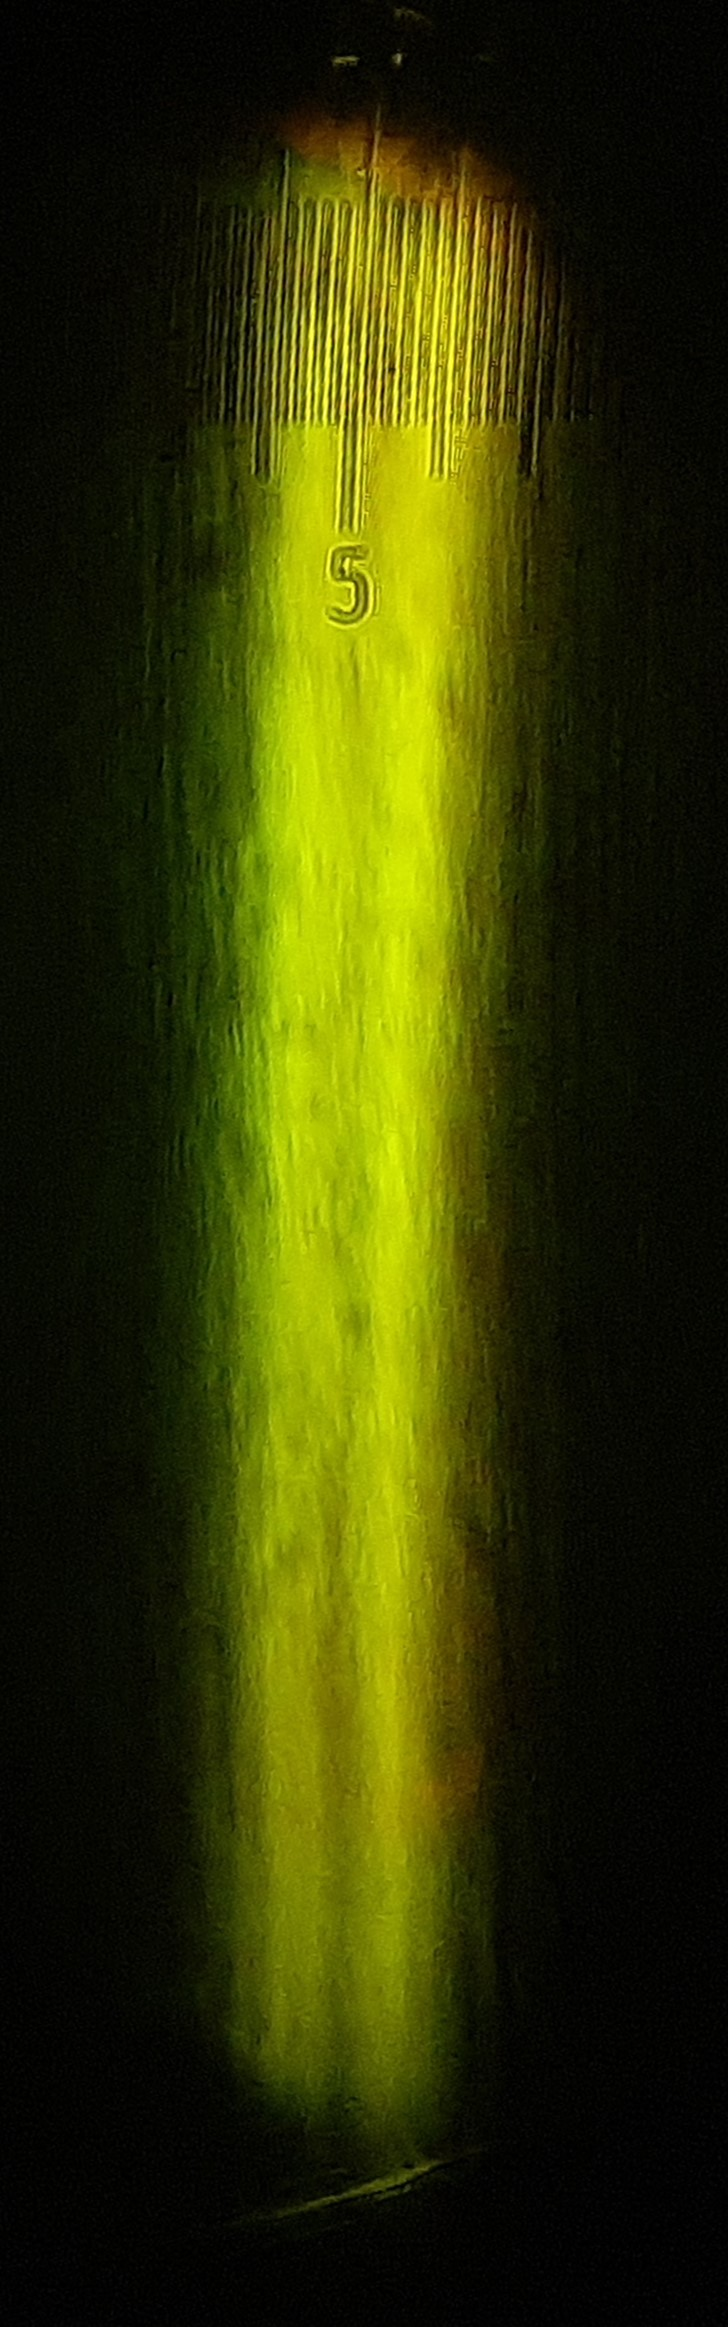
\includegraphics[width=.75\linewidth]{../images/431m_2}
\end{minipage}%
\begin{minipage}{.33\textwidth}
  \centering
  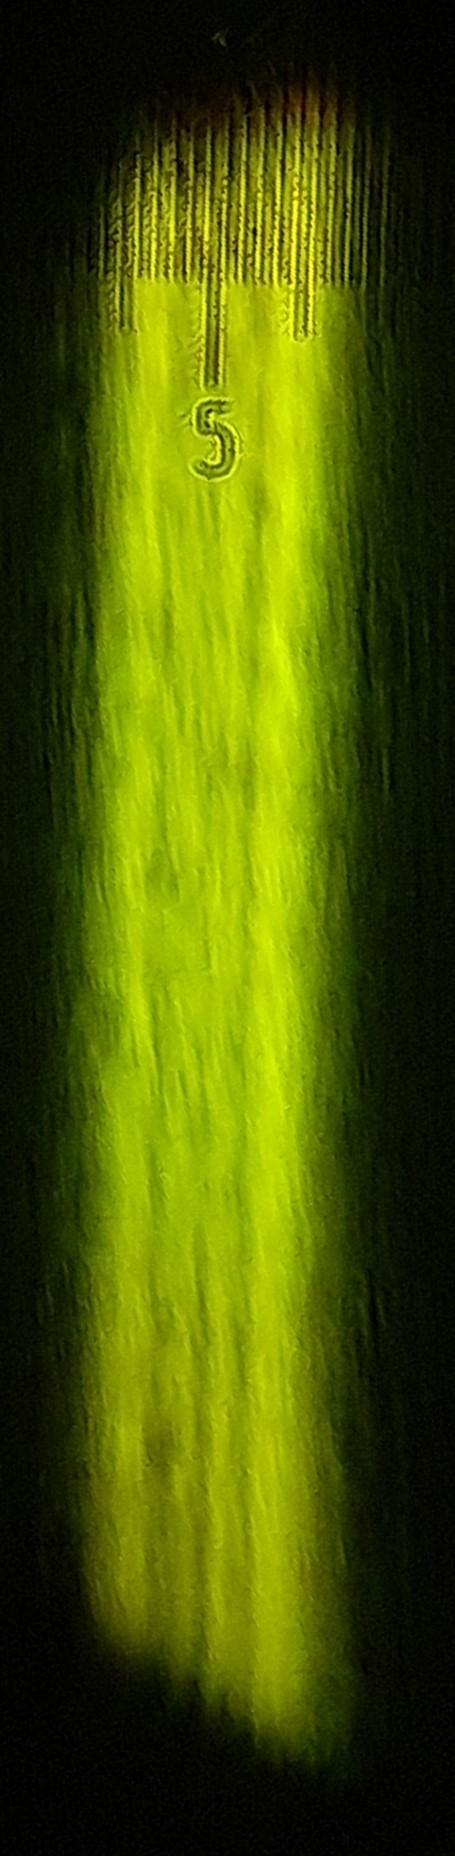
\includegraphics[width=.6\linewidth]{../images/431m_3}
\end{minipage}%
\begin{minipage}{.33\textwidth}
  \centering
  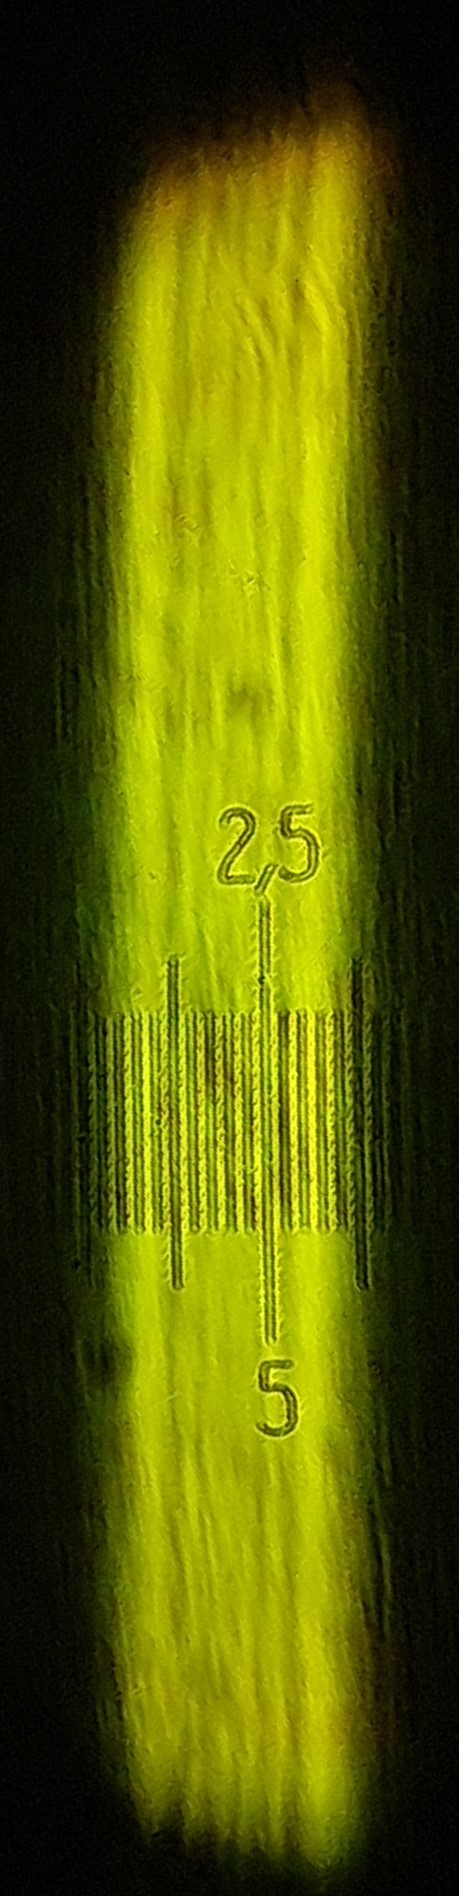
\includegraphics[width=.6\linewidth]{../images/431m_4}
\end{minipage}
\end{figure}

\item Приближая микроскоп к щели, измерим зависимость координаты микроскопа от числа наблюдаемых темных полос.

\item Измерим ширину щели $S_2$, используя окулярную шкалу микроскопа ($b=1.5\ мм$).

\end{enumerate}

\section{Обработка результатов}

\begin{enumerate}

\item Подберем координаты так, чтобы зависимость расстояния до щели от числа открытых зон Френеля была линейной.

\item Построим график зависимости $m(1/z)$ и аппроксимируем прямой линией.

\begin{figure}[H]
\centering
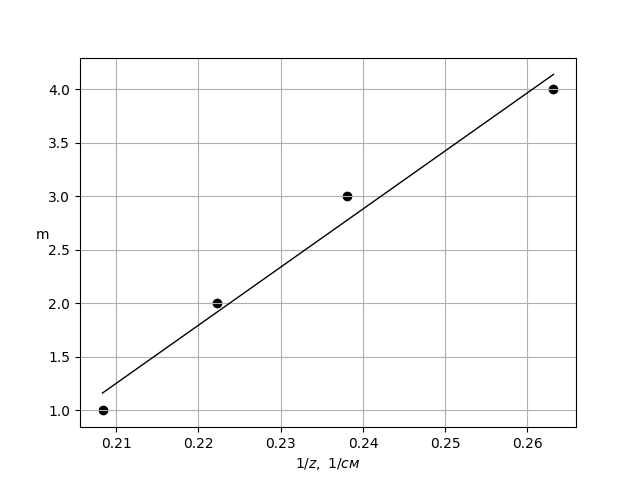
\includegraphics[scale=0.6]{../images/431m_6}
\end{figure}

\item По наклону прямой $a$ определим ширину щели.

\[b=2\sqrt{a\lambda}\approx1.1\ мм\]

\end{enumerate}

\paragraph*{Б. Дифракция Фраунгофера на щели}

\section{Настройка установки}

\begin{enumerate}

\item Не разбирая схемы из прошлого эксперимента, добавим к ней линзу между щелью $S_2$ и микроскопом.

\item Настроим микроскоп на фокальную плоскость линзы.

\item Подберем ширину щели $S_2$ так, чтобы в поле зрения появилась дифракционная картина.

\begin{figure}[H]
\centering
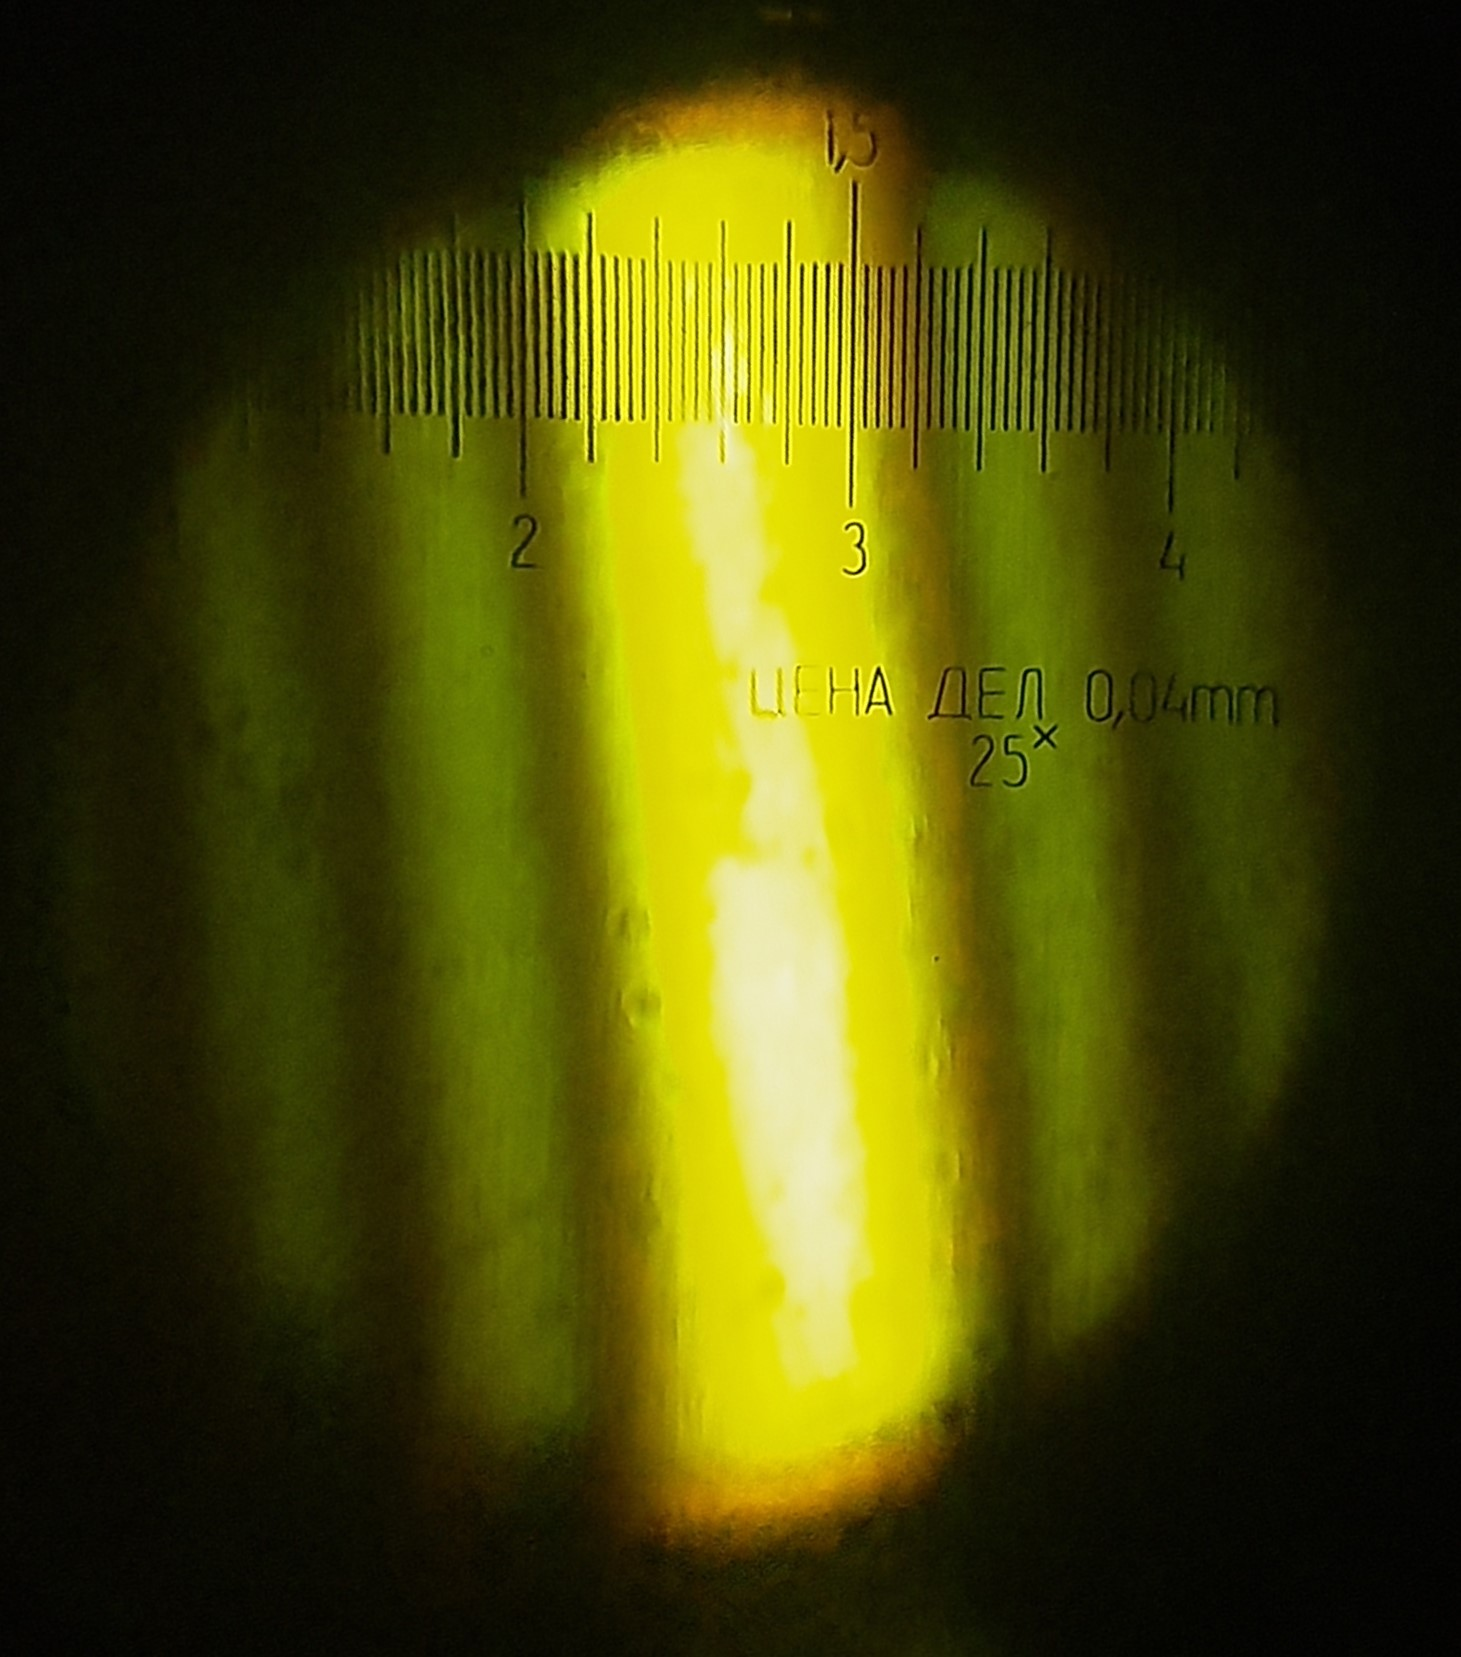
\includegraphics[scale=0.2]{../images/431m_5}
\end{figure}

\end{enumerate}

\section{Проведение измерений}

\begin{enumerate}

\item Измерим с помощью окулярной шкалы микроскопа координаты нескольких дифракционных минимумов в обе стороны от центра.

\item Запишем ширину щели $S_2$ и фокусное расстояние линзы ($b=0.15\ см$, $f=10\ см$).

\end{enumerate}

\section{Обработка результатов}

\begin{enumerate}

\item Построим график зависимости положений экстремумов дифракционной картины от их номера. Убедимся, что зависимость может быть аппроксимирована прямой линией.

\begin{figure}[H]
\centering
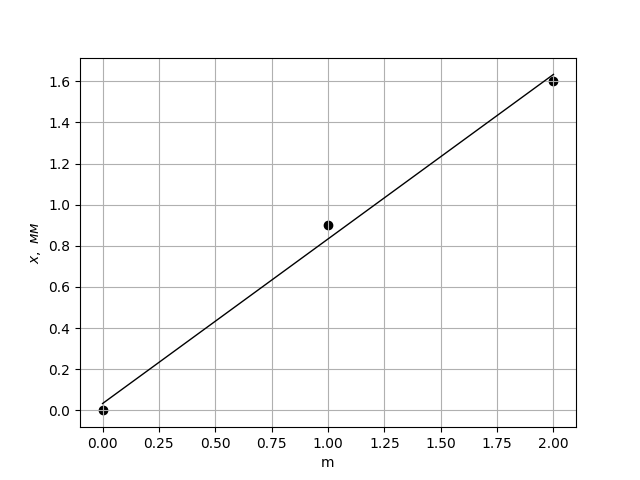
\includegraphics[scale=0.6]{../images/431m_7}
\end{figure}

\item По наклону прямой $a$ определим ширину щели $S_2$.

\[b=\frac{f\lambda}{a}\approx0.07\ мм\]

\end{enumerate}

\section{Выводы}

В ходе проведенной лабораторной работы были исследованы явления дифракции Френеля и Фраунгофера и проверены теоретические соотношения для положения максимумов при дифракции Френеля и Фраунгофера.

\end{document}